%*****************************************
\chapter{Preparation}\label{ch:preparation}
%*****************************************

In this chapter we formulate the objectives presented in Section \ref{sec:objectives} into a set of design principles, drawing on existing work. We justify the use of broadcast encryption and define a suitable scheme. We describe possible deployment strategies and briefly review Firefox extension development and the Facebook platform. We also look at the specific problems associated with encrypting images and draft a security policy. Finally, we derive a concrete set of requirements and outline an appropriate software development methodology and testing plan


\FloatBarrier
\section{Design principles}
\label{sec:principles}

We begin by outlining several key principles which were used to constrain the rest of the design and development process. We briefly describe how they enforce the stated aims of privacy preservation, scalability, usability and incremental deployment and how they relate to existing solutions. Note that here use of the term third-party excludes Facebook itself.


\FloatBarrier
\subsection{Encryption of shared content}

It is possible to preserve privacy by encrypting or otherwise concealing the link between a real life user and their online identity. This is the basis of NOYB \cite{noyb}. Arguably, however, privacy is only poorly preserved due to problems of inference control \cite{ross}.\footnote{An obvious example is that many users will be easily identifiable simply from the photos they upload.} Incremental deployment is also hampered since non-users can't see the real names of the users they interact with \cite{facecloak}.

The alternative is to encrypt shared content itself in some way or another, restricting access to only those who possess the appropriate key even in the event of exposure.


\FloatBarrier
\subsection{Independence from third-party servers}

In addition to using encryption, flyByNight, FaceCloak and uProtect.it opt to migrate content from the Facebook platform to an external third-party database.

We consider the practice of outsourcing content to conflict with our stated goal of scalability. Storing and delivering encrypted content requires at least the resources needed for storing and delivering the cleartext. Facebook are currently able to offer a free service by serving highly targeted advertising to members based on the structure of the social graph \cite{fb-ads}. This revenue stream would be largely unavailable to any solution hosting a database of encrypted content.

Third-party servers can also be employed for performing encryption and/or decryption (as with uProtect.it and flyByNight) or as part of a public key infrastructure. Again, the resources required by the server would scale linearly in proportion to the amount of content exchanged.


\FloatBarrier
\subsection{Secret key security}

Any encryption scheme will require some form of key whose secrecy is required.

It is possible to use a trusted third-party to store and distribute secret keys in a so-called key escrow arrangement. Key management can even be taken out of the users hands entirely, improving usability. This is the basis of uProtect.it \cite{uprotect}. However, confidentiality is only weakly assured since trust has simply been deferred from Facebook to the third-party and many of the scenarios raised in Section \ref{sec:background} still apply.

Another possibility is using secret keys derived from a password. flyByNight, for example, allows users to download a password-protected private key from their server. We could also store password protected keys in-band (i.e. on Facebook itself) or generate a key simply by hashing a password. Relying on the user to memorize a password rather than manage secret keys also improves usability. Unfortunately the entropy of user chosen passwords is far less than that of randomly generated keys \cite{passwords}.

By ensuring we use randomly generated keys that are only ever stored on the user's device(s) we trade usability for better privacy protection. Appropriate key lengths are discussed in Section \ref{ssec:keys}.


\FloatBarrier
\subsection{Minimal use of OOB channels}

Secure OOB (out-of-band) channels\footnote{Such as encrypted email or face-to-face exchange.} can be used to transmit content, update messages, keys or other information as part of an encryption scheme. Since these channels are, by definition, external to the Facebook platform it can be hard to automate such exchanges and much is still required from the user. FaceCloak, for example, requires users to transmit messages over secure email when adding friends. The process is partly automated, however the user must set up an email client and install and configure PGP themselves \cite{facecloak}.

By limiting the use of OOB transmission we mitigate usability concerns regarding manual key management. The exception is when installing a secret key across more than one device --- since transporting a secret key by any other means would compromise the principle of secret key security.


\FloatBarrier
\section{One-to-many communication}

Communication over social networks is typically one-to-many whereas cryptography traditionally considers one sender and a single recipient. We look at existing solutions and outline the broadcast encryption scheme we adopted for Encrypted Facebook.


\FloatBarrier
\subsection{Existing solutions}
\label{ssec:exist}

uProtect.it, flyByNight and FaceCloak tackle this problem in the following ways:

\begin{enumerate}

    \item If content is both hosted and encrypted/decrypted remotely, as with uProtect.it, one-to-many support is trivial. The user simply authenticates with the server and is sent the cleartext.
    
    \item If a third-party is able to perform computation a technique called proxy re-encryption can be used, as with flyByNight \cite{flybynight}. Here the server changes the key under which the content may be decrypted on demand, without ever being able to read the cleartext itself \cite{proxy}.
    
    \item Distributing keys over OOB channels can permit one-to-many communication. A FaceCloak user, for example, shares a single decryption key OOB among friends \cite{facecloak}.

\end{enumerate}

(1) and (2) are incompatible with the design principle of third party independence, whilst (3) violates the principle of limited OOB channel use.

\FloatBarrier
\subsection{Broadcast encryption}

An alternative to the solutions in Section \ref{ssec:exist} is to use a broadcast encryption\footnote{Broadcast encryption is defined in Appendix \ref{app:bcast}.} scheme. 

In general, schemes can be characterised by the size of each user's private and public key and the amount of transmission overhead that must be sent with each message, given the number of recipients. The scheme we use here has a relatively large transmission overhead, however unlike other more complex schemes it doesn't require the use of key-update messages. Transmitting key-updates OOB or though a third-party would violate our stated design principles. Transmitting them in-band would be possible, but since Facebook is a best-effort service synchronisation and lost updates would likely be a problem.

Let $U$ be the set of users with Encrypted Facebook installed and $R \subseteq U$ be a set of intended recipients. For simplicity we describe broadcast encryption as a key encapsulation mechanism:


\begin{defn}
    
    Given a suitable asymmetric encryption scheme $P$ and a suitable symmetric scheme $Q$, we define our broadcast encryption scheme as the triple of algorithms {\sc (Setup, Broadcast, Decrypt)} such that:
    
    \begin{itemize}
    
    \item {\sc (Setup)} takes a user $u \in U$ and constructs their private key $priv_u$ and public key $pub_u$ using scheme $P$.
    
    \item {\sc (Broadcast)} takes the list of privileged users $R$, generates a session key $k$ using scheme $Q$ and broadcasts a message $b$ where:
    
    \begin{itemize}
        \item $b$ is the list of pairs $(u,k_u)$ such that $u \in R$, where $k_u$ is the session key encrypted under $pub_u$.
    \end{itemize}
    
    
    \item A user $u \in U$ runs {\sc Decrypt($b, u, priv_u$)} that will:
    
        \begin{itemize}
            \item If $(u,k_u) \in b$, extract the session key $k$ from $k_u$ using $priv_u$.
        
            \item {\sc Decrypt} fails, if $(u,k_u) \notin b$ or if, equivalently, $u \notin R$.
        
        \end{itemize}

    \end{itemize}
    
\end{defn}    

\cite{survey} provides a proof that this scheme is at least as secure as the underlying encryption schemes $P$ and $Q$. A more advanced scheme which also doesn't require key-updates is proposed in Appendix \ref{ssec:bcast-improved} and discussed in Section \ref{sec:future}. It was not pursued initially because it was thought that a working implementation couldn't be guaranteed.


\FloatBarrier
\section{Intercepting Facebook interactions}

In order to encrypt content it must be intercepted before being submitted to Facebook. We describe the possible places at which this can occur (Figure \ref{fig:approaches})) and briefly justify the approach we took with Encrypted Facebook.

\subsection{Possible deployment strategies}

\begin{figure}[tb]
\begin{center}
    \pgfdeclarelayer{device}
\pgfdeclarelayer{browser}
\pgfdeclarelayer{sandbox}
\pgfdeclarelayer{fg}
\pgfsetlayers{device,browser,sandbox,fg,main}
\begin{tikzpicture}[
    every node/.style={font={\footnotesize \bfseries}, minimum width=0.5cm, text centered, thick, black!80},
    box/.style={rounded corners, draw=black!50, dashed}
]

%draw web page
\node (a1) at (0,5) {};
\node (b1) [on grid,below=1cm of a1] {};
\node (c1) [on grid,below=1cm of b1] {};
\node (d1) [on grid,below=1cm of c1] {};

\node[fit=(a1) (d1)] (page1) {};
\node[text width=2em] at (page1) (page2) {Web page};
\begin{pgfonlayer}{fg}
    \node[draw,  fill=green!20, fit=(page1) (page2)] (page3) {};
\end{pgfonlayer}


%draw entires
\node[draw,fill=white,minimum width=0.7cm,minimum height=0.5cm] (a2) [on grid,right=6cm of a1] {a};
\node[draw,fill=white,minimum width=0.7cm,minimum height=0.5cm] (b2) [on grid,right=4.4cm of b1] {b};
\node[draw,fill=white,minimum width=0.7cm,minimum height=0.5cm] (c2) [on grid,right=3.2cm of c1] {c};
\node[draw,fill=white,minimum width=0.7cm,minimum height=0.5cm] (d2) [on grid,right=2cm of d1] {d};

% boxes
\node[fit= (page3) (a1) (d1) (d2) ] (sandbox1) {};
\node[below] at (sandbox1.south) (sandbox2) {Sandbox};
\begin{pgfonlayer}{sandbox}
    \node[box, fill=blue!10, fit= (sandbox1) (sandbox2) ] (sandbox3) {};
\end{pgfonlayer}

\node[fit=(sandbox3) (c2)] (browser1) {};
\node[below] at (browser1.south) (browser2) {Browser};
\begin{pgfonlayer}{browser}
    \node[box, fill=blue!5, fit=(browser1) (browser2) ] (browser3) {};
\end{pgfonlayer}

%and client
\node[draw,fill=white,minimum width=0.7cm,minimum height=0.5cm] (e1) [on grid,below=4cm of browser3] {e};

\node[fit=(e1)] (client1) {};
\node[below] at (client1.south) (client2) {Facebook client};
\begin{pgfonlayer}{browser}
    \node[box, fill=blue!5, fit=(client1) (client2)] (client3) {};
\end{pgfonlayer}

% draw facebook
\node (a3) [on grid,right=8cm of a1] {};
\node (b3) [on grid,below=1cm of a3] {};
\node (c3) [on grid,below=1cm of b3] {};
\node (d3) [on grid,below=1cm of c3] {};
\node (e3) [on grid,right=7cm of e1] {};

\node[fit=(a3) (e3)] (fb1) {};
\node at (fb1) (fb2) {Facebook};
\begin{pgfonlayer}{fg}
    \node[draw=black!50, fill=green!20, fit=(fb1) (fb2)] (fb3) {};
\end{pgfonlayer}

\node[fit=(browser3) (b2) (client3)] (device1) {};
\node[below] at ($(device1.south)+(0,-0.5cm)$) (device2) {User device};
\begin{pgfonlayer}{device}
    \node[box, fill=yellow!20, fit=(device1) (device2)] (device) {};
\end{pgfonlayer}

\path[name path=ppath] (page3.north east) -- (page3.south east);
\path[name path=fpath] (fb3.north west) -- (fb3.south west);

% arrows
\foreach \x in {a,b,c,d} {
    \path[name path=a12] (\x 1) -- (\x 2);
    \draw [->,name intersections={of=a12 and ppath, by=x}]
    [thick, black!80] (\x 2) -- (x);
    
    \path[name path=a23] (\x 2) -- (\x 3);
    \draw [<-,name intersections={of=a23 and fpath, by=x}]
    [thick, black!80] (x) -- (\x 2);
}

\path[name path=eee] (e1) -- (e3);
\draw [<->,name intersections={of=eee and fpath, by=x}]
[thick, black!80] (x) -- (e1);



\end{tikzpicture}
\caption{Possible deployment strategies for intercepting interaction with Facebook.}
\label{fig:approaches}
\end{center}
\end{figure}


\begin{enumerate}
\renewcommand{\labelenumi}{\alph{enumi})}
    
    \item On a remotely hosted proxy server. Provides easier multi-OS and multi-browser support.
    
    \item On a proxy server running on localhost. Providers easier multi-browser support.
    
    \item Within the browser, outside the browser sandbox. Extensions and plugins exist here and have elevated privileges over normal site code. Other examples include signed Java applets, ActiveX controls and to a lesser extent inline Flash and Silverlight applications.\footnote{Flash applications, for example, are restricted but can provide basic filesystem access \cite{flash-sbox}.} FaceCloak takes this approach.
    
    \item Within the browser, entirely inside the browser sandbox - using only JavaScript and HTML. uProtect.it and flyByNight both take this approach.
    
    \item Outside the browser as part of a bespoke Facebook client application.
    
\end{enumerate}
   
Approach (a) would conflict with the design principle of third party independence. The browser sandbox prevents local filesystem access, ruling out (d) if private keys are generated and stored securely. We took approach (c) since (b) and (e) are considerably more complex, at some cost to cross-platform compatibility.



\FloatBarrier
\section{Mozilla Firefox extension development}
\label{sec:ffox}

The project was developed as an extension for Mozilla Firefox, the world's most popular browser (as of January 2011). Manipulating the DOM (Document Object Model) is well supported by browser extensions since the browser interface chrome is often built on existing web technologies. Porting to other browsers is discussed in Section \ref{sec:deploy}.

Firefox extensions are written in JavaScript with partial support for binding library code written in Python or C/C++. Performing cryptography in JavaScript is possible but comes with severe performance difficulties \cite{flybynight}. Table \ref{tab:lang-speeds} compares approximate performance for each language based on some provisional tests.


\begin{figure}[tb]
\begin{center}
\begin{tabular}{+l ^l ^l}
    \rowstyle{\bfseries}%
    Language & Library & Time (ms) \\
    \midrule
    Python 2.6.6 & pycryptopp 0.5.17 & 1,220 ms \\ [1ex]
    C++ 98 & Botan 1.8.11 & 92 ms \\ [1ex]
    \parbox[t][][t]{20ex}{\raggedright JavaScript 1.6 (in Chrome 12.0.712)} & \parbox[t][][t]{20ex}{\raggedright JavaScrypt (last updated December 2005)} & 1,685,000 ms \\
\end{tabular}
\caption{Approximate time for 256-bit AES encryption of 1000 1.5 MiB random messages.}
\label{tab:lang-speeds}
\end{center}
\end{figure}

Since long delays would hamper usability we opted to use C/C++ for computation intensive operations. Native code can be executed from within Firefox in three ways:

\begin{itemize}

    \item Creating an XPCOM component. These are linked against a single Gecko\footnote{Gecko is the layout engine used by Firefox.} version; supporting multiple versions is possible but non-trivial \cite{xpcomm}.
    
    \item Loading native libraries with {\tt js-ctypes}. Introduced in Gecko 2.0 \cite{js-ctypes}. 

    \item Using {\tt nsiProcess} to invoke an external stand-alone application. Capturing output can be difficult.
    
\end{itemize}

Since building an entire XCPOM component would be excessive and give little advantage by way of multi-version compatibility, the newly introduced {\tt js-ctypes} module was used to load native code. This restricted us to Firefox version 4.0 and above, however Gecko 2.0 also has the advantage of providing better support for working with the local filesystem and manipulating images in the DOM.


\FloatBarrier
\section{The Facebook platform}
\label{sec:facebook}

%Facebook represents the social graph as objects and connections between them. Objects include users, photos, messages and events. All objects are assigned a single unique Facebook ID and all objects (except users themselves) are associated with the ID of the user who created them (their owner). The owner's privacy settings (global and per object) will partly determine who may access an object. Objects will also have connections to other users and other objects. For example, users can create discussion threads by commenting on objects or tag other users as being present in a photograph.

Facebook represents all entities (e.g. users, messages, photos, events) uniformly as nodes in the social graph. Each node has a unique Facebook ID, several attributes including an object type, and one or more connections to other nodes.\footnote{This is actually a slight simplification. For full details refer to the Facebook Graph API reference documentation.}

We make the generalisation that interaction with Facebook amounts to creating and retrieving objects in the social graph. Our goal then is to encrypt and decrypt the attributes of certain object types - the body of a message object, for example. We do not attempt to encrypt or otherwise conceal connections between objects; this is an non-goal as stated in Section \ref{sec:limit}.

We describe the most popular forms of object submitted and discuss issues relating to the connectedness of user nodes and the signal-to-noise ratio in network feeds. We then briefly look at interfacing with the Facebook platform.

\FloatBarrier
\subsection{Content types}
\label{sec:content}

Encrypting all possible types of object would be prohibitively complex. Ideally we should encrypt those most frequently used. From the data available these are Comments, Messages, Images and Posts (Table \ref{tab:fb-activities}). 

Without relying on a third-party server all transmission overheads must be stored on Facebook itself, in one form or another. Images and blog-style notes are obvious targets for storage utilisation due to their large capacity (see Table \ref{tab:fb-activities}). In particular, the body of a note can contain over 120 KiB of information since each character represents one 16-bit Unicode code point. Images are subject to lossy compression which is discussed in Section \ref{ssec:images}.

\begin{table}[tb]
  \begin{center}
        \definecolor{lgrey}{hsb}{0.1, 0, 0.9}
        %\rowcolors{3}{white}{lgrey}
        \begin{tabular}{+l ^l ^l}
            \rowstyle{\bfseries}%
            Activity & Frequency  & Limitations \\
            \rowstyle{\bfseries}%
            & (per second) & \\
            \midrule
            Comment         & 8,507    & 8,000 chars.   \\ 
            Message         & 2,263    & 10,000 chars.  \\
            Image           & 2,263    & $720 \times 720$ pixels \\  
            Friend request  & 1,643    &                \\
            Status update   & 1,320    & 420 chars.     \\
            Wall post       & 1,323    & 1,000 chars.   \\
            Event invite    & 1,237    &                \\
            Photo tag       & 1,103    &                \\
            Link            & 833      &                \\
            Note            & Unknown  & 65,536 chars.  \\
        \end{tabular}
        \caption{Facebook objects and connections, their limitations and approximate frequency of creation \cite{fb-stats}}
        \label{tab:fb-activities}
    \end{center}
\end{table}

Each user's profile has a "Bio"\footnote{Sometimes referred to as the "About me" field.} field with a character limit of 64,536. With no other capacious attribute that can be easily queried from a user ID this is the obvious place to store a user's public key.

    
\subsection{Connectedness}
\label{sec:cness}

Since broadcast encryption has a transmission overhead proportional to the number of intended recipients, care must be taken to ensure the system works with large enough recipient groups. The number of recipients is bounded by the number of friends a user or equivalently by the degree of the user's node in the social graph. Empirical estimates for the average number of Facebook friends range from 130 to 170, with some evidence suggesting the distribution drops off sharply at around 250 \cite{fb-factsheet} \cite{fb-connectedness}.

The Dunbar number is a theoretical cognitive limit to the number of people a user can maintain relationships with and has been applied to social networks as well as face-to-face interactions. Estimates range from around 150 to 300 \cite{dunbar} \cite{socnetsize}, suggesting that average node degree is unlikely to increase dramatically as Facebook expands further.


\subsection{Signal-to-noise ratio}
\label{sec:signoise}

Activity within the social graph causes notifications to be posted to feeds. The news feed, for example, is shown to users on logging in (Figure \ref{scn:fbook}  We define the signal-to-noise ratio of a feed as the proportion of useful items to non-useful items.\footnote{By non-useful items we typically mean spam, but in our case this could be transmission overheads as part of the broadcast encryption scheme or even the encrypted content itself.}

In order to permit incremental deployment any system must ensure that its users can coexist with non-users. Ideally the impact on signal-to-noise ratio should be limited.

    \begin{figure}[tb]
        \begin{center}
                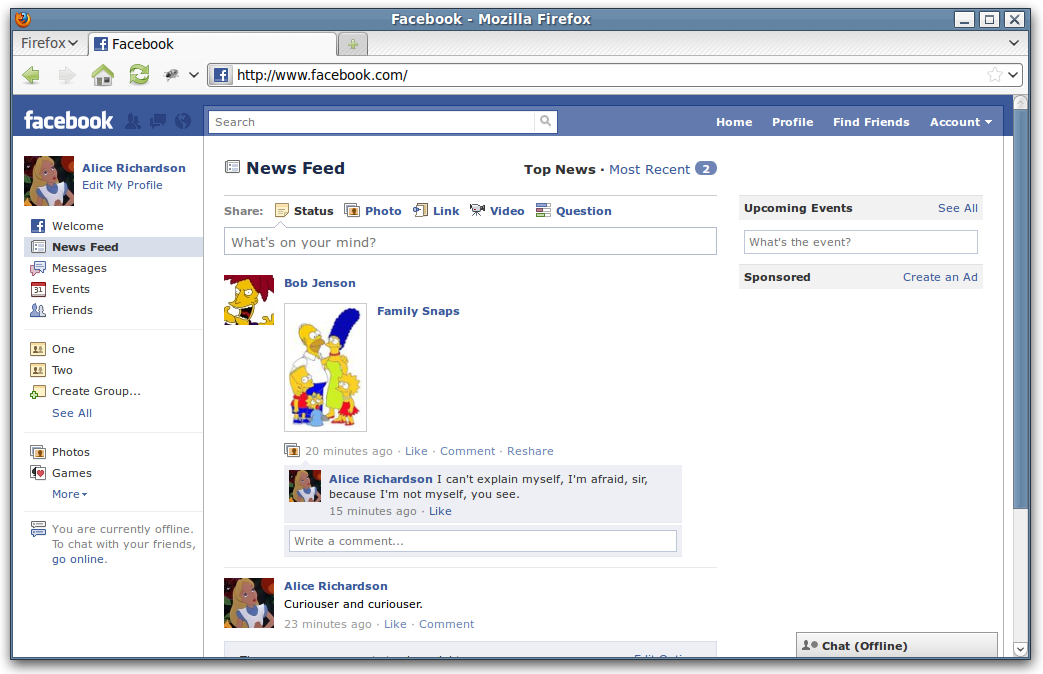
\includegraphics[width=12cm]{screens/facebook.png}
            \caption{News feed as presented on login.}
            \label{scn:fbook}
        \end{center}
    \end{figure}

\FloatBarrier
\subsection{Graph API}

Facebook does provide a JavaScript SDK for interfacing with the Facebook platform, however it is poorly documented and doesn't allow uploading images - since most JavaScript applications are designed to run inside the browser sandbox without local filesystem access. Instead, we may use the Facebook Graph API directly.

Authentication is performed using the OAuth 2.0 protocol. Applications register with Facebook and present their application ID upon request. The user then confirms that the application may use the requested permissions and an access token is generated. This token is then used in future exchanges.

Unfortunately some actions\footnote{Namely working with the local filesystem and modifying the "Bio" attribute.} are poorly supported by the Graph API, if at all. Appendix \ref{app:graph} describes the API in more detail, as well as the required workarounds.

    
\FloatBarrier
\section{Encrypting images}
\label{ssec:images}

%As well as being one of the most frequently used types of content, images have been highlighted as a prime privacy concern on social networks \cite{fb-images}. None of the existing work supports image encryption, though flyByNight discusses it as a possible extension.

Regardless of the input format, Facebook encodes all uploaded images using lossy JPEG.\footnote{Even if a file is already in the output format the compression process is repeated and information is lost.} We therefore require some form of JPEG-immune coding for the binary output of encryption, so that after undergoing compression we can exactly recover the original bytes.

Appendix \ref{app:images} describes Facebook's JPEG compression process. To motivate the need for a more complex scheme we evaluate two naive attempts at encoding data in images, before proposing a more advanced approach. Note that we only consider greyscale images.\footnote{Chrominance subsampling means RGB images provide a less than 50\% increase in capacity over greyscale. See Appendix \ref{app:images}.}


\subsection{Naive data insertion}
\label{ssec:naive}

One approach would be to encode directly into greyscale pixel values with enough redundancy to overcome the information lost during compression. A second might be to similarly encode data into the DCT coefficients of an existing JPEG image, since through the process of decompression and re-compression only a small amount of information is lost. The main source of information loss for the second approach is from capping DCT coefficients which don't map back to greyscale values in the range 0-255.

\begin{figure}[tbph]
  \begin{center}
\begin{tikzpicture}
    \begin{axis}[grid=major,xlabel=JPEG Quality Factor,ylabel=BER (\%), xmin=80, xmax=90,
    height=8cm,width=10cm,legend style={legend pos=north east}]
    
    \addplot
        table[x=QF,y=rgb] {gfx/error_rate0.data};
    \addplot
        table[x=QF,y=dct] {gfx/error_rate0.data};
    \legend{Pixels,DCT}
    
    \end{axis}
\end{tikzpicture}
    \caption{Bit error rate for varying quality factors.}
    \label{graph:ber0}
  \end{center}
\end{figure}

Figure \ref{graph:ber0} graphs the bit error rate for both methods over a range of quality factors, using the IJG (Independent JPEG Group) {\tt libjpeg} library for compression. Quality factor 85 most closely matches the compression signature used by Facebook (see Appendix \ref{app:images}). For encoding in DCT coefficients a special bitmask, generated from the quantisation matrix, is used in an attempt to reduce the incidence of capping (see Appendix \ref{app:dct} for details). Modelling the compression process as a binary symmetric channel, Figure \ref{graph:capacity0} graphs the theoretical per-image capacity of each method for lossless data transmission (details for this calculation are given in Evaluation Section \ref{ssec:capacity}).


\begin{figure}[tbph]
  \begin{center}
\begin{tikzpicture}
    \begin{axis}[grid=major,xlabel=JPEG Quality Factor,ylabel=Capacity (KiB/image), xmin=80, xmax=90,
    height=8cm,width=10cm,legend style={legend pos=north west}]
    
    \addplot
        table[x=QF,y=rgb2] {gfx/error_rate0.data};
    \addplot
        table[x=QF,y=dct2] {gfx/error_rate0.data};
    \legend{Pixels,DCT}
    
    \end{axis}
\end{tikzpicture}
    \caption{Per-image channel capacity (measured in KiB/image) for varying quality factors.}
    \label{graph:capacity0}
  \end{center}
\end{figure}

Given a recipient group size of 400 and a ciphered session key size of 1024-bit (see Section \label{ssec:keys}) the transmission overhead alone would be at at least 50 KiB.\footnote{50 KiB not including the list of recipient IDs, initialisation vector and any padding or size tags.} A $720 \times 720$ image encoded at low quality (IGJ quality factor 10) would still require around 25 KiB of storage space \cite{ijg}. This means neither of the naive approaches would be suitable even given an error correction scheme which performs at or near the Shannon limit. 


\subsection{Advanced data insertion}

One initial optimisation for any coding scheme would be to map binary data to appropriate length grey codes to ensure that only single bit errors occur from erroneously outputting an adjacent codeword. In addition, we present two possible schemes, henceforth referred to as the HWT (Haar Wavelet Transform) method and the n-bit scaling method.

\begin{sdesc}

    \item[HWT method] \hfill \\ JPEG DCT compression selectively quantises perceptually redundant high frequency components. Wavelet transforms allow us to embed data in the low frequency sub-band of the carrier signal and can be performed reversibly by using an integer lifting scheme. Xu et al demonstrate that data encoded in low-frequency HWT approximation coefficients can survive JPEG decompression when combined with an error correction scheme \cite{haar}.
    
    \item[N-bit scaling method] \hfill \\ This method maps the n-bit input space on to the 8-bit pixel space by scaling the input by a factor of $ \frac{2^8 - 1}{2^n - 1}$. The inverse process amounts to outputting which interval pixel value lies in. This method works on the assumption that large changes in single pixel intensity are unlikely to occur due to compression.

\end{sdesc}

Clearly both these schemes are sub-optimal and their exact properties (compression time and error rates) are unknown. We made it a requirement that the project should take a modular approach to conduit image implementations: firstly to ensure that both of the proposed schemes can be implemented simultaneously and their performances compared; secondly, to aid future development of a more optimal solution.



\FloatBarrier 
\section{Security Policy}
\label{sec:security}

To truly protect privacy we must consider proper security engineering practices. Of particular concern is introducing new vulnerabilities into the browser platform. We perform a threat analysis and describe issues relating to the underlying cryptographic scheme.

\FloatBarrier
\subsection{Threat analysis}
\label{ssec:threat}

The threat analysis is included in its entirety in Appendix \ref{app:threat}. We take an attack-centric approach, defining risk as $Vulnerability \times Threat \times Impact$ according the methodology described by \cite{security}. Below we summerise several potential threats and possible counter measures, proportionate to the risk posed:


\begin{sdesc} \addtolength{\itemsep}{-0.5\baselineskip}
    \item[Attack 1] Attacker breaks the encryption scheme by brute force methods.
    \item[Measures] Ensure key sizes are appropriate given the type of attacker. See Section \ref{ssec:keys}.
\end{sdesc}

\begin{sdesc} \addtolength{\itemsep}{-0.5\baselineskip}
    \item[Attack 2] Attacker gains access to user's computer through the download and execution of a file.
    \item[Measures] Ensure only legitimate JPEG and public key files are downloaded. Public key files can be vetted on their character set and size, JPEG's by their extension.
\end{sdesc}

\begin{sdesc} \addtolength{\itemsep}{-0.5\baselineskip}
    \item[Attack 3] Attacker gains access to user's computer by injecting code into {\tt eval()} which runs outside the browser sandbox.
    \item[Measures] Wrap all calls to {\tt eval()} with a {\tt secureEval()} function which attempts to prevent malicious use. 
\end{sdesc}

\begin{sdesc} \addtolength{\itemsep}{-0.5\baselineskip}
    \item[Attack 4] Attacker gains access to Facebook account through browser code injection.
    \item[Measures] Sanitize all user inputs and ensure sanitisation can't be bypassed e.g. through the UTF-8 decoder\cite{utf8}. Also sanitize output whenever inserting code into the DOM.
\end{sdesc}

\begin{sdesc}\addtolength{\itemsep}{-0.5\baselineskip}
    \item[Attack 5] Attacker carries out middle-person attack by intercepting and switching public keys.
    \item[Measures] Informing the user whenever public keys are updated removes a large amount of risk. Complete protection would be impractical without use of OOB channels.
\end{sdesc}

\begin{sdesc} \addtolength{\itemsep}{-0.5\baselineskip}
    \item[Attack 6] Attacker causes DoS by creating a malicious object.
    \item[Measures] This need not be a large problem since decryption is built to fail gracefully (see Section \ref{ssec:ident-targets}). Include some simple run time checks to limit iteration and special characters (combined with proper sanitisation) to prevent tags-within-tags.
\end{sdesc}


\FloatBarrier
\subsection{Underlying encryption schemes}
\label{ssec:keys}

NIST(National Institute of Standard and Technology) publish guidelines on cryptographic schemes and protocols. Since 2010 NIST have recommended using at least 128-bits of security \cite{nist-key}.

The ideal scheme would be based on elliptic curve cryptography since comparable strength public keys are much smaller than for finite field or integer factorisation methods (see Table \ref{tab:keys}). This is important since the block size of the cipher depends on the public key; this in turn determines the size of the transmission overhead. Unfortunately ECC is less common in open libraries due to patent concerns.

\begin{table}[tbph]
  \begin{center}
        \definecolor{lgrey}{hsb}{0.1, 0, 0.9}
        %\rowcolors{3}{white}{lgrey}
        \begin{tabular}{+l ^l ^l ^l}
            \rowstyle{\bfseries}%
            Bits of Security & FFC & IFC & ECC \\
            \midrule
            80 &  1024  & 1024 & 160-223 \\
            112 & 2048  & 2048 & 224-255 \\
            128 & 3072  & 3072 & 256-383 \\
            192 & 7680  & 7680 & 384-511 \\
            256 & 15360 & 15360 & 512+ \\
        \end{tabular}
        \caption{Table of public key length equivalences \cite{nist-key}}
        \label{tab:keys}
    \end{center}
\end{table}

We opted to use RSA and AES due to their wide availability in libraries like Botan. Given the possible advantages of using ECC we made it a requirement that the cryptographic components of the library be extensible. This also accommodates for future increases in key lengths, perhaps due to revised recommendations. 


\FloatBarrier
\section{Requirements specification}
\label{sec:req}

Based on the contents of this chapter we derive a set of concrete requirements.
        
\begin{desc}

    \item[Requirement 1] The extensions will be able to broadcast-encrypt, submit, retrieve and decipher the following objects:
    
    \begin{itemize}
        \item Status updates
        \item Wall posts
        \item Comments
        \item Messages
        \item Images
    \end{itemize}
    
    \item[Requirement 2] The size limits for encrypted text objects will be no smaller than the current limits Facebook imposes, given in Section \ref{sec:content}).

    \item[Requirement 3] The size limit for encrypted images will be no less than 50 KiB. This is roughly equivalent to a $720 \times 720$ image encoded at medium quality (IJG quality factor 25) \cite{ijg}.

    \item[Requirement 4] To ensure the goal of scalability is met, all requirements will be met given recipient groups sizes up to 400, based on the discussion in Section \ref{sec:cness}.
    
    
    \item[Requirement 5] To ensure the goal of usability is met, all response times will lie within acceptable limits, in accordance with \cite{response}.


    \item[Requirement 6] To ensure privacy is protected, the project will adhere to the security policy described in \ref{ssec:threat}.


    \item[Requirement 7] The number of news feed entries generated by encrypted submission will be no more than the number generated by normal content submission. This ensures that the effect on signal-to-noise ratio is kept to an absolute minimum - the only perceivable 'noise' is the encrypted content itself.
    

    \item[Requirement 8] There are uncertainties and/or trade-offs associated with certain approaches to encryption and encoding data in images (and to a lesser extent error correction). It is also clear that in some cases the optimal approach is well beyond the scope of this project. Therefore, we make it a requirement to adopt a modular structure that facilitates switching between differing schemes and permits future extension.
    
\end{desc}


   
\FloatBarrier 
\section{Development}
        
An agile development style was adopted loosely based on \cite{agile}. Uncertainties in the optimal approach or combination of approaches for encryption, image coding and error correction meant that being flexible and able to respond to changes was crucial. Delivering functional prototypes at various stage in the development life-cycle also fits with the project's modularity requirement. In addition, since the bulk of the project concerns encapsulating data in some layer of encoding the natural approach would be to build successive prototypes, each implementing a new layer.

\subsection{Development environment}

Git was used for revision control and backup. The working repository is stored on a laptop and pushed twice-daily to a remote repository hosted by ProjectLocker.

Komodo edit was used as a development IDE, as recommended by Mozilla. C++ coding style followed the GeoSoft guidelines \cite{code-style} and documentation was generated automatically using Doxygen.

Firefox 4.0 pre-beta was obtained through APT by adding the Mozilla Daily Build Team PPA. The build process consists of compiling and linking the C++ shared library, then packaging this (together with the rest of the extension code) and automatically installing to a number of Firefox development profiles.        

GNU Octave (a free MATLAB-like application) was also used for provisional evaluation and to generate some of the results in this section.


\subsection{Testing plan}

We loosely adopt the agile testing principles of test driven development rather than a test last approach. Ensuring the feedback loop between testing and implementation is kept as short as possible allows us to maintain flexibility, which is useful given the uncertainties over the optimal image approach.

Special attention needed to be made to security relevant testing such as input sanitisation and proper functioning of the UTF-8 decoder. Boundary-value analysis was used to generate sets of test scripts (included in Appendix \ref{app:bv}).

To help ensure the goal of usability was met, usability testing in the form of cognitive walkthroughs were performed. During development many passes of the walkthroughs were performed and alterations made, until a credible success story could be constructed for each task. Excerpts from final success stories are presented in Section \ref{sec:use}.

